\newcommand{\uSubset}{U_S}
\newcommand{\oSubset}{O_S}
\newcommand{\UAExpr}{UAExpr}
\newcommand{\OAExpr}{OAExpr}
\newcommand{\uSelector}{USERs}
\newcommand{\oSelector}{OBJECTs}
\newcommand{\policySpace}{PolicySpace}

  \begin{table} 
\centering
\caption{One abstract policy represented by different \sABAC{} policies}
\label{table:sabac-def}
\begin{tabular}{@{}l@{}}
 \toprule	
	 $  E(role(u), \{manager, employee\}) \land E(type(o),\{new\} )$\\
	 $  E(role(u), \{manager\}) \land E(role(u), \{employee\}) \land E(type(o),\{new\} )$\\
	 $ \lnot E(role(u), \{\}) \land E(role(u), \{employee\}) \land E(type(o),\{new\} )$\\
 	 $ \lnot (\lnot (E(role(u), \{manager, employee\}))) \land E(type(o),\{new\} )$\\
 \bottomrule
\end{tabular}
\end{table}
 
 \textbf{Abstract Policy}
 We define abstract policy as a tuple of following forms - $(\uSubset, a, \oSubset)$ and $(\UAExpr, a, \OAExpr)$, where $\uSubset \subseteq U$ and $\oSubset \subseteq O$, $\uSelector(\UAExpr) \subseteq U$ and $\oSelector(\OAExpr) \subseteq O$, for function $\uSelector()$ and $\oSelector()$ which specifies set of users and objects for given user attribute expression and object attribute expression. Examples of abstract policy are $(\{ Alice, Bob\}, read, \{ o1, o2\} )$ or $( E(role(u), \{manager \}), read, E(\{ type(o), \{sensitive\} ) ) $
 
 We say two abstract policies $\rho_i \equiv (\UAExpr_i, a, \OAExpr_i)$ and   $\rho_j \equiv (\UAExpr_j, a, \OAExpr_j)$ are different ($\rho_i \neq \rho_j$) iff either or both of following conditions are true.
 \begin{enumerate}
 	\item $\uSelector(\UAExpr_i) \neq  \uSelector(\UAExpr_j) \lor U_i \neq U_j$  
 	\item $\oSelector(\OAExpr_i) \neq  \oSelector(\OAExpr_j) \lor O_i \neq O_j$
 \end{enumerate}

Informally, \policySpace{} of an model is the set of all distinct abstract policies of the model. For simplicity, here we are only interested about the size of the \policySpace{}.

	\begin{figure} 
		\centering
		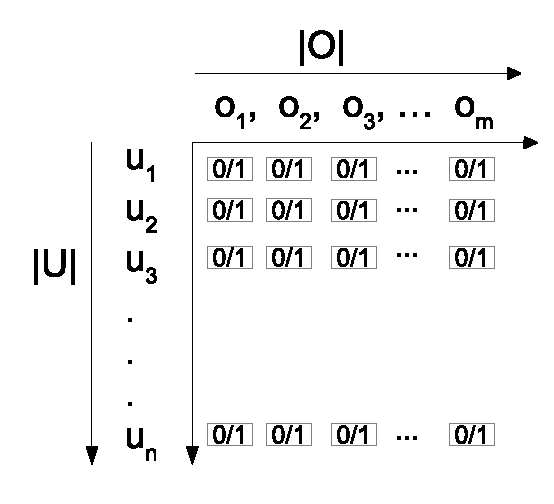
\includegraphics[width=.4\textwidth]{policyspace-hru}
		\caption{LaBAC with one object label and one user label}
		\label{fig:policyspace-hru}
	\end{figure}
 	\begin{figure} 
 		\centering
 		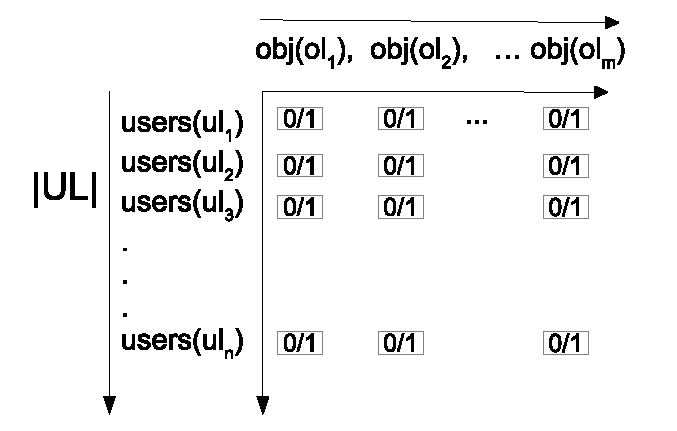
\includegraphics[width=.4\textwidth]{policyspace-labac1}
 		\caption{LaBAC with one object label and one user label}
 		\label{fig:policyspace-labac1}
 	\end{figure}
 	\begin{figure} 
 		\centering
 		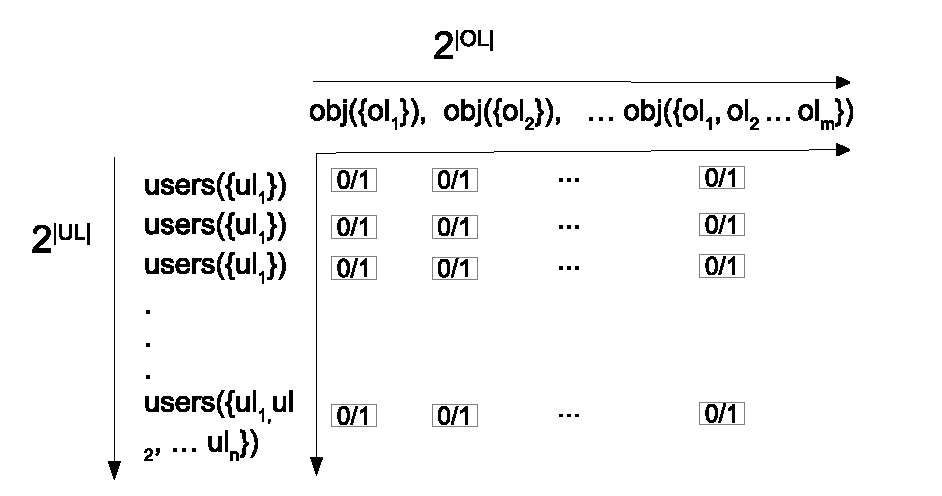
\includegraphics[width=.4\textwidth]{policyspace-labace}
 		\caption{LaBAC with one object label and one user label}
 		\label{fig:policyspace-labace}
 	\end{figure}
% Please add the following required packages to your document preamble:
 % \usepackage{booktabs}
 \begin{table}
 	\centering
 	\caption{Comparison of \policySpace{}}
 	\label{tab:policyspace-comparison}
 	\begin{tabular}{|l|l|}
 		 \hline
 		\textit{HRU \cite{hru}} & $ 2 ^{|U| \times |O|}$ \\
 		\textit{\labacOneOneOne{} } & $ 2 ^{|UL| \times |OL|}$ \\
 		\textit{\elabac} & $ 2 ^{2^{|UL|} \times 2^{|OL|}}$ \\
 		\textit{$\abacAlpha{} \cite{abacAlpha}$} & $2 ^{32}$ \\
 		\textit{\hgabac{}* \cite{hgabac}} & $ 2 ^{2^{|ua_1|} \times 2^{|oa_1|}}$ \\
\hline
 	\end{tabular}
 \end{table} 
